\documentclass[10pt, compress]{beamer}

\usetheme{m}

\usepackage{booktabs}


\title{FEM/DGM Coupling}
\subtitle{MSc 1 Projet Report}
\date{Year 2014-2015}
\author{Mathieu Gaborit}
\institute{Université du Maine}

\begin{document}

\maketitle

\begin{frame}[fragile]
  \frametitle{Initial state}
  \begin{columns}[onlytextwidth]
    \column{0.6\textwidth}

      \begin{itemize}
        \item Numerous numerical methods, each with specificities
        \item Proven efficiency of methods relying on adaptative meshes
        \item A powerful adaptative method yet to be found
      \end{itemize}

    \column{0.4\textwidth}\centering
        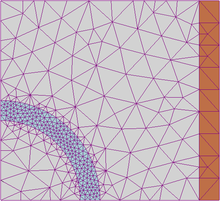
\includegraphics[width=\textwidth]{mesh.png}
  \end{columns}

\end{frame}

\section{Methods}

\begin{frame}[fragile]
    \frametitle{Wave-based DGM \& FEM}

    \begin{block}{Wave-based Discontinuous Galerkin Method}
    \begin{itemize}
       \item Use of a \alert{plane-waves basis} to improve accuracy
       \item Number of unknowns only dependent on the \alert{number of plane waves} in the test-field
       \item Excellent approximation event for \alert{huge elements} with big details
    \end{itemize}
    \end{block}

    \begin{block}{Finite Elements Method}
    \begin{itemize}
       \item Number of unknowns dependent on the \alert{order of the chosen polynomials}
       \item Excellent approximation for small elements with \alert{tiny details}
       \item \alert{Robust} and used for years
    \end{itemize}
    \end{block}
\end{frame}

\begin{frame}
    \frametitle{How to mix ?}

    \begin{center}
        Problem to solve : \alert{Write the interface operator} !
    \end{center}

    \begin{itemize}
        \item Write boundary conditions for FEM using characterics-based formulation from DGM
        \item Choose wisely the polynomial basis to preserve order while applying boundary conditions
        \item Solve the meshing discontinuity problem (between TR6 and TR3 meshes)
        \item Snap all that together and pray !
    \end{itemize}
\end{frame}

\begin{frame}
    \frametitle{What's done, what's left ?}

    \begin{block}{Done}
        \begin{itemize}
            \item Test of different polynomial basis for FEM
            \item FEM computation using characterics-based boundary conditions
            \item Simple 1D-DGM computation
        \end{itemize}
    \end{block}
    \pause
    \begin{block}{Still to do}
        \begin{itemize}
            \item Coupling of FEM and DGM
            \item Evaluation of method accuracy for simple problems
            \item Reflexion around 2D generalization of the method
        \end{itemize}
    \end{block}
\end{frame}

\begin{frame}
    \frametitle{References}

    \begin{itemize}
        \item \textbf{A discontinuous Galerkin Method with Plane Waves for Sound Absorbing Materials}, \textit{Int. J.
            Numer. Engng}, G. Gabard, O.  Dazel
        \item \textbf{A comparison of wave-based discontinuous Galerkin, ultra-week and least-square method for wave
            problems}, \textit{Int. J.
            Numer. Engng}, G. Gabard, P. Gamallo, T. Huttunen
        \item \textbf{Analyse Numérique : une approche mathématique}, M. Schatzman
    \end{itemize}
\end{frame}

\end{document}
